% !TEX root = ../../main.tex
 
\chapter{Vorfeldanalyse (\Jai)}
 
\section{Anforderungen und Abgrenzung}
 
\subsection{Anforderungen an die Infrastruktur}
 
Die Lernplattform wird von Lernenden einer Schule benutzt. Meistens sind nur wenige Personen gleichzeitig online. Vor Schularbeiten, Tests und Abgaben sind es aber viel mehr (Eig.)\footnote{„Eig.“ kennzeichnet in diesem Kapitel eigene Einschätzungen ohne gesonderten Quellenbeleg.}. Die Infrastruktur muss auch diese Spitzen aushalten. Aus dem Projektantrag und den Rahmenbedingungen ergeben sich diese Anforderungen:
 
\begin{itemize}
  \item Die Plattform läuft auf einem Server der Schule. Wenn die Schule keinen Server bereitstellen kann, läuft sie lokal auf einem eigenen Rechner.
  \item Die Serverumgebung lässt sich jederzeit gleich neu aufbauen und bei Bedarf vergrößern.
  \item Die Struktur der Datenbank wird konzipiert und definiert, das heißt, welche Daten es gibt und wie sie zusammenhängen.
  \item Eine relationale Datenbank ist angebunden und arbeitet zuverlässig mit dem Backend zusammen.
  \item Die Anmeldung läuft zentral über ein Active Directory. Weil die Schule keinen Zugriff auf ihr eigenes Active Directory gibt, wird dafür ein eigenes eingerichtet.
  \item Lerninhalte können strukturiert importiert und exportiert werden.
  \item Das System ist abgesichert, die Daten werden gesichert und können wiederhergestellt werden. Bei einem Ausfall läuft die Plattform möglichst weiter.
  \item Sicherheit, Geschwindigkeit, Belastbarkeit und Stabilität werden getestet und die Ergebnisse dokumentiert.
\end{itemize}
 
\subsection{Abgrenzung zu Backend und Frontend}
 
Das Gesamtprojekt besteht aus Backend, Frontend und Infrastruktur. Die Infrastruktur stellt die Umgebung bereit, in der Backend und Frontend laufen. \Luca entwickelt die Backend-Logik, den adaptiven Lernalgorithmus und die API. \Jakob entwickelt die Benutzeroberfläche. \\ \\
Bei der Anmeldung über das Active Directory sind die Aufgaben so aufgeteilt: Die Einstellungen im Django-Backend gehören zum Backend. Die Infrastruktur liefert das Verzeichnis, die Netzwerkverbindung, die Zertifikate und Testkonten. Bei der Datenbank legt die Infrastruktur die Struktur fest, also Tabellen, Beziehungen und Regeln. Die Umsetzung im Backend, also die Django-Modelle und Migrationen, gehört zu \Luca. Der Betrieb des Datenbankservers, die Backups und die Verfügbarkeit gehören ebenfalls zur Infrastruktur. Die genauen Schnittstellen werden im Infrastrukturkonzept festgehalten (Meilenstein am 15.11.2026).
 
 
\section{Begrifflichkeiten}
 
\begin{center}
\begin{tabular}{|p{4.2cm}|p{9.5cm}|}
\hline
\textbf{Begriff} & \textbf{Erklärung} \\ \hline
Active Directory (AD) & Verzeichnisdienst von Microsoft, der Benutzer:innen und Gruppen in einem Netzwerk verwaltet \\ \hline
LDAP / LDAPS & Protokoll, mit dem man ein Verzeichnis abfragen und Anmeldungen prüfen kann. LDAPS ist die verschlüsselte Version \\ \hline
Container & Eine Art Paket, in dem eine Anwendung mit allem läuft, was sie braucht \\ \hline
Docker Compose & Programm, mit dem man mehrere Container gemeinsam beschreibt und mit einem Befehl startet \\ \hline
Git / Repository & Versionsverwaltung für Dateien. Im Repository liegen der Code und die Konfigurationen, hier auf GitHub \\ \hline
Reverse Proxy & Server vor der Anwendung, der Anfragen annimmt und an die Anwendung weiterleitet \\ \hline
Horizontale / vertikale Skalierung & Mehr Instanzen starten bzw. einen stärkeren Server verwenden \\ \hline
Primärschlüssel / Fremdschlüssel & Der Primärschlüssel kennzeichnet eine Zeile in einer Tabelle eindeutig. Ein Fremdschlüssel verweist auf eine Zeile in einer anderen Tabelle \\ \hline
ER-Diagramm & Zeichnung der Datenbank mit Tabellen (Entitäten) und ihren Beziehungen \\ \hline
Migration & Beschreibung einer Änderung an der Datenbankstruktur, die sich in Django automatisch ausführen lässt \\ \hline
Transaktion & Mehrere Datenbankänderungen, die entweder ganz oder gar nicht ausgeführt werden \\ \hline
Backup & Sicherungskopie der Daten, aus der man sie wiederherstellen kann \\ \hline
Lasttest / Stresstest & Test mit erwarteter Last bzw. mit mehr Last, als das System aushalten soll \\ \hline
DSGVO & Datenschutz-Grundverordnung der EU \\ \hline
\end{tabular}
\end{center}
 
\section{Serverinfrastruktur und Datenbank}
 
\subsection{Reproduzierbarkeit und Container}
 
Reproduzierbar heißt, dass sich die ganze Serverumgebung jederzeit aus einer Beschreibung neu aufbauen lässt. Die Einstellungen werden nicht von Hand am Server gemacht, sondern stehen in Dateien, die versioniert werden. So kann man jede Änderung nachvollziehen, und der Server kann bei einem Problem einfach neu erstellt werden. \\
Dafür werden Container mit Docker verwendet. Ein Container enthält die Anwendung und alles, was sie zum Laufen braucht. Dadurch läuft sie überall gleich. Mit Docker Compose werden mehrere Container gemeinsam beschrieben und mit einem Befehl gestartet. Bei uns sind das zum Beispiel der Reverse Proxy, die Django-Anwendung und die Datenbank. Die Beschreibung liegt zusammen mit dem Code in einem Git-Repository auf GitHub. Die Anwendung kann damit auf einem neuen Server geklont und gestartet werden. Geheime Daten wie Passwörter liegen nicht im Repository, sondern in Umgebungsvariablen. Es gibt auch größere Werkzeuge wie Kubernetes. Sie bringen aber viel Aufwand mit und sind für ein Projekt dieser Größe nicht nötig (Eig.).
 
 
\subsection{Skalierbarkeit und Reverse Proxy}
 
Skalierbar heißt, dass das System auch mit mehr Benutzer:innen gut funktioniert. Es gibt zwei Wege. Bei der vertikalen Skalierung bekommt der Server stärkere Hardware. Bei der horizontalen Skalierung laufen mehrere Instanzen der Anwendung. Dafür dürfen die Instanzen keine Daten bei sich selbst speichern, sie müssen zustandslos sein. Sitzungen und Dateien liegen dann in der Datenbank, in einem gemeinsamen Cache oder in einem gemeinsamen Speicher \parencite[Kap.~1 und 5]{kleppmann2017}.
Vor den Instanzen steht ein Reverse Proxy, zum Beispiel nginx. Er nimmt die Anfragen an, kümmert sich um die verschlüsselte Verbindung (TLS) und leitet sie an die Anwendung weiter. Laufen mehrere Instanzen, verteilt er die Anfragen auf sie. Django läuft im Betrieb nicht mit dem eingebauten Testserver, sondern mit einem Produktionsserver wie Gunicorn. \\
Daraus ergibt sich der Aufbau in Schichten: Browser, Reverse Proxy, Django-Anwendung und Datenbank. Dazu kommen das eigene Active Directory und die Orte, an denen die Backups liegen (siehe Abbildung~\ref{fig:architektur}).
\begin{figure}[htbp]
  \centering
  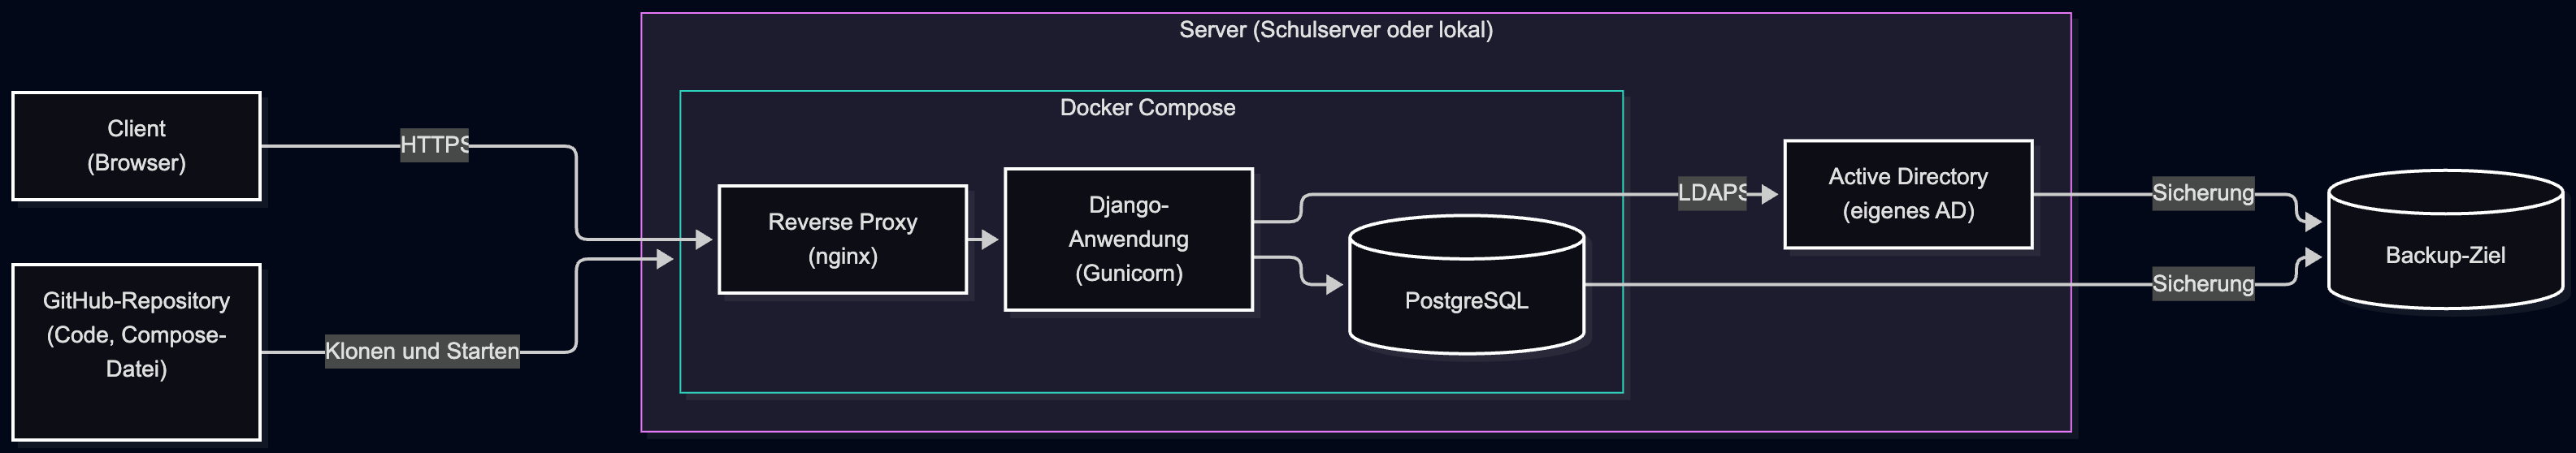
\includegraphics[width=\textwidth,height=0.45\textheight,keepaspectratio]{Bilder/Kumar/Architekturübersicht.png}
  \caption{Architekturübersicht der Infrastruktur (eigene Darstellung)}
  \label{fig:architektur}
\end{figure}
 
\subsection{Relationale Datenbank}
 
Die Plattform speichert viele Daten, die zusammenhängen: Benutzer:innen, Lerninhalte, Lernkarten, Tests, Ergebnisse und Wiederholungstermine. Dafür passt eine relationale Datenbank gut. Sie sorgt über Fremdschlüssel dafür, dass die Verbindungen zwischen den Daten stimmen. Mit Transaktionen wird verhindert, dass ein Ergebnis nur halb gespeichert wird, wenn mitten im Vorgang ein Fehler passiert. Django kann mit mehreren relationalen Datenbanken arbeiten. Für das Projekt ist PostgreSQL vorgesehen, weil es gut mit Django zusammenarbeitet und gute Möglichkeiten für Backups bietet. \\
Die Datenbank läuft in einem eigenen Container. Ihre Daten werden außerhalb des Containers gespeichert, damit sie beim Neustart nicht verloren gehen. Die Zugangsdaten stehen in Umgebungsvariablen und nicht im Code. Außerdem ist die Datenbank nur für die Anwendung erreichbar und nicht von außen.
 
\section{Datenbankstruktur}
 
\subsection{Aufgabe und Vorgehen}
 
Neben der Serverinfrastruktur konzipiert und definiert \Jai die Struktur der Datenbank. Gemeint ist, welche Daten gespeichert werden, in welche Tabellen sie aufgeteilt sind und wie die Tabellen zusammenhängen. Die Umsetzung im Backend, also die Django-Modelle und Migrationen, bleibt bei \Luca. Damit beide Seiten dasselbe meinen, wird die Struktur schriftlich festgehalten. Das Vorgehen ist so geplant:
 
\begin{enumerate}
  \item Aus den Anforderungen werden die Daten gesammelt, die gespeichert werden müssen.
  \item Die Daten werden in Entitäten (spätere Tabellen) gegliedert, und es wird festgelegt, wie sie zusammenhängen.
  \item Für jede Tabelle werden Schlüssel, Pflichtfelder und Regeln festgelegt, zum Beispiel was beim Löschen passiert.
  \item Das Ergebnis wird als ER-Diagramm und als Tabellenbeschreibung dokumentiert.
  \item Die Struktur wird mit \Luca und \Jakob abgestimmt und nach der Umsetzung der ersten Modelle mit dem echten Code verglichen.
\end{enumerate}
 
Als Ausgangspunkt dient der Entwurf der Entitäten in der Vorfeldanalyse von \Luca. Dieser wird hier weiterentwickelt.
 
\subsection{Grundbegriffe}
 
Eine relationale Datenbank speichert Daten in Tabellen. Jede Zeile ist ein Datensatz und wird durch einen Primärschlüssel eindeutig gekennzeichnet. Beziehungen zwischen Tabellen werden mit Fremdschlüsseln ausgedrückt. Gehören viele Datensätze zu genau einem anderen, zum Beispiel viele Lernkarten zu einem Lerninhalt, spricht man von einer 1-zu-n-Beziehung. Können viele Datensätze mit vielen anderen verbunden sein, zum Beispiel viele Benutzer:innen mit vielen Lernkarten, braucht man eine Zwischentabelle. Django bildet ein Modell, also eine Python-Klasse, in der Regel auf eine Tabelle ab, und Beziehungen werden mit einem \texttt{ForeignKey} ausgedrückt \parencite{djangoModels}. Eine einfache Grundregel beim Entwurf ist, jede Information nur an einer Stelle zu speichern. Dann kann sie sich nicht widersprechen (Eig.).
 
\subsection{Entwurf der Datenbankstruktur}
 
Aus den Anforderungen ergeben sich die Tabellen in der folgenden Übersicht. Die Aufteilung ist ein Entwurf, und einzelne Felder können sich bei der Umsetzung noch ändern.
 
\begin{center}
\small
\begin{tabular}{|p{3.0cm}|p{5.6cm}|p{5.0cm}|}
\hline
\textbf{Tabelle} & \textbf{Inhalt} & \textbf{Beziehungen} \\ \hline
Benutzer & Person, die die Plattform nutzt, mit einer Rolle (Lernende, Lehrkraft, Administration) & Hat Testversuche, Lernergebnisse und Wiederholungsstatus \\ \hline
Lerninhalt & Thema des Lernstoffs, das Lernkarten und Tests bündelt & Hat mehrere Lernkarten und Tests \\ \hline
Lernkarte & Karte mit Frage und Antwort & Gehört zu einem Lerninhalt \\ \hline
Test & Zusammenstellung von Testaufgaben zu einem Lerninhalt & Gehört zu einem Lerninhalt, hat mehrere Testaufgaben \\ \hline
Testaufgabe & Einzelne Frage eines Tests mit der Lösung & Gehört zu einem Test \\ \hline
Testversuch & Ein Durchlauf eines Tests durch eine Person mit Zeitpunkt und Gesamtergebnis & Gehört zu einem Benutzer und einem Test \\ \hline
Lernergebnis & Bewertung einer einzelnen Antwort mit Zeitpunkt & Gehört zu einem Benutzer und zu einer Lernkarte oder Testaufgabe \\ \hline
Wiederholungs-\newline status & Aktueller Planungszustand einer Lernkarte für eine Person, zum Beispiel der nächste Wiederholungstermin & Verbindet Benutzer und Lernkarte (Zwischentabelle) \\ \hline
\end{tabular}
\end{center}
 
Die Beziehungen sind in Abbildung~\ref{fig:er} als ER-Diagramm dargestellt. Der Lernfortschritt wird nicht als eigene Tabelle gespeichert, sondern aus den Lernergebnissen und dem Wiederholungsstatus berechnet. Dadurch kann er den gespeicherten Daten nicht widersprechen (Eig.). Passwörter von Benutzer:innen aus dem Active Directory werden nicht in der Datenbank gespeichert, denn sie liegen im Verzeichnis.
 
\begin{figure}[htbp]
  \centering
  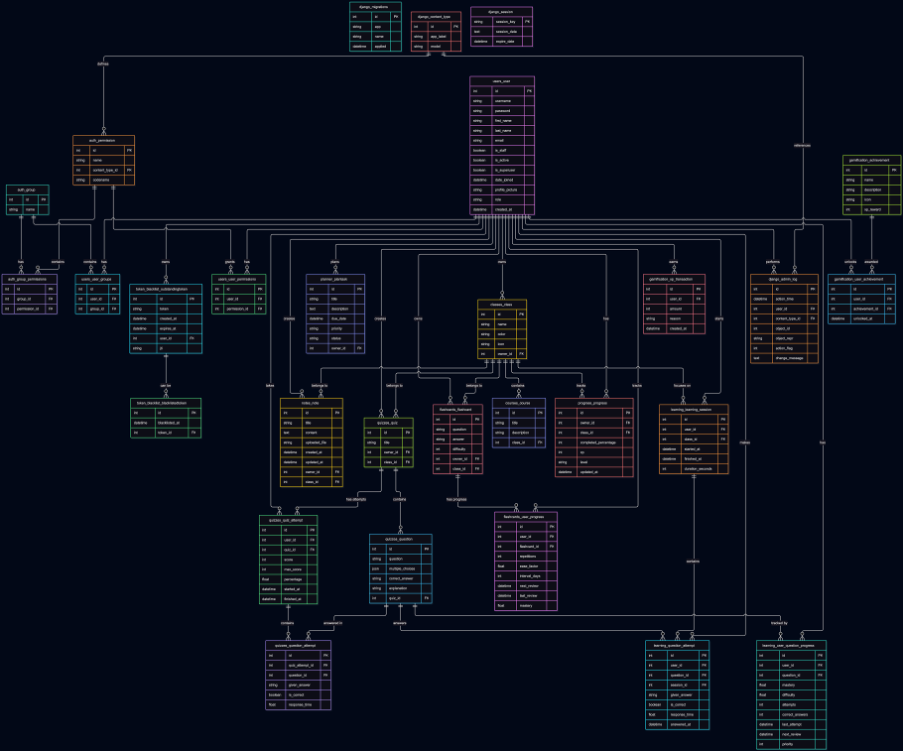
\includegraphics[width=\textwidth,height=0.45\textheight,keepaspectratio]{Bilder/Kumar/ER_Diagramm.png}
  \caption{Entwurf der Datenbankstruktur als ER-Diagramm (eigene Darstellung)}
  \label{fig:er}
\end{figure}
 
\subsection{Regeln und Leistung}
 
Zusätzlich zu den Tabellen werden Regeln festgelegt, die die Datenbank selbst überwacht:
 
\begin{itemize}
  \item \textbf{Eindeutigkeit:} Pro Benutzer:in und Lernkarte gibt es höchstens einen Wiederholungsstatus. Die Datenbank stellt das sicher.
  \item \textbf{Löschverhalten:} Wird ein Benutzer gelöscht, werden die dazugehörigen Lernergebnisse, Testversuche und Wiederholungsstatus mitgelöscht oder anonymisiert. Welche Variante gewählt wird, hängt vom Datenschutz ab und ist noch offen.
  \item \textbf{Zusammengehörige Änderungen:} Ein Lernergebnis und der neue Wiederholungsstatus werden in einer Transaktion gespeichert, damit nie nur eines von beiden gespeichert wird \parencite{djangoTransactions}.
  \item \textbf{Geschwindigkeit:} Die häufigste Abfrage ist vermutlich die nach den fälligen Lernkarten einer Person. Dafür kann ein Index sinnvoll sein, der solche Abfragen beschleunigt \parencite[Kap.~3]{kleppmann2017}. Ob er nötig ist, zeigen die Performancetests.
  \item \textbf{Änderungen:} Änderungen an der Struktur laufen über Migrationen, die zusammen mit dem Code im Repository liegen. So lässt sich jede Änderung nachvollziehen (Eig.).
\end{itemize}
 
\section{Active-Directory-Anbindung}
 
\subsection{Verzeichnisdienste und Protokolle}
 
In Schulnetzwerken verwaltet normalerweise ein Active Directory (AD) die Konten, Gruppen und Passwörter. Wenn eine Lernplattform ein solches Verzeichnis benutzt, müssen sich Lernende nicht neu registrieren und kein zusätzliches Passwort merken. Konten müssen nur an einer Stelle gepflegt werden. Wird ein Konto deaktiviert, zum Beispiel nach dem Schulaustritt, gilt das auch für die Plattform. \\
Für dieses Projekt bekommt das Team keinen Zugriff auf das AD der Schule. Deshalb wird ein eigenes Active Directory eingerichtet. Es läuft auf dem Server neben der Anwendung und enthält Testkonten für Lernende und Lehrende. Für die Anwendung ändert sich dadurch nichts Grundsätzliches, denn die Anmeldung funktioniert wie beim Schul-AD. Falls später doch ein Zugriff auf das Schul-AD möglich wäre, müssten im Wesentlichen nur die Einstellungen angepasst werden. \\
Die Anwendung spricht mit dem AD über das Protokoll LDAP. Sie nimmt Benutzername und Passwort entgegen und prüft sie beim Verzeichnis (siehe Abbildung~\ref{fig:ad}). Dabei sind diese Punkte wichtig:
 
\begin{itemize}
  \item \textbf{Verschlüsselung:} Passwörter dürfen nicht unverschlüsselt übertragen werden. Deshalb wird LDAPS verwendet.
  \item \textbf{Service-Account:} Ein technisches Konto mit möglichst wenigen Rechten sucht die Benutzer:innen im Verzeichnis.
  \item \textbf{Gruppen und Rollen:} AD-Gruppen, zum Beispiel für Lernende und Lehrende, können Rollen in der Plattform bekommen.
  \item \textbf{Ausfall:} Wenn das AD nicht erreichbar ist, soll nicht die ganze Plattform stillstehen. Deshalb braucht es einen Notfallzugang für Administrierende.
\end{itemize}
 
 
\subsection{Anbindung an Django}
 
Für Django gibt es das Paket \emph{django-auth-ldap}, das die Anmeldung über LDAP übernimmt. Laut Dokumentation prüft es Benutzer:innen gegen einen LDAP-Dienst und kann Benutzer, Gruppen und Berechtigungen verwalten \parencite{django-auth-ldap}. Die Einstellungen im Backend macht \Luca. Das eigene Verzeichnis, die Netzwerkverbindung und die Zertifikate stellt die Infrastruktur bereit.
 
\begin{figure}[htbp]
  \centering
  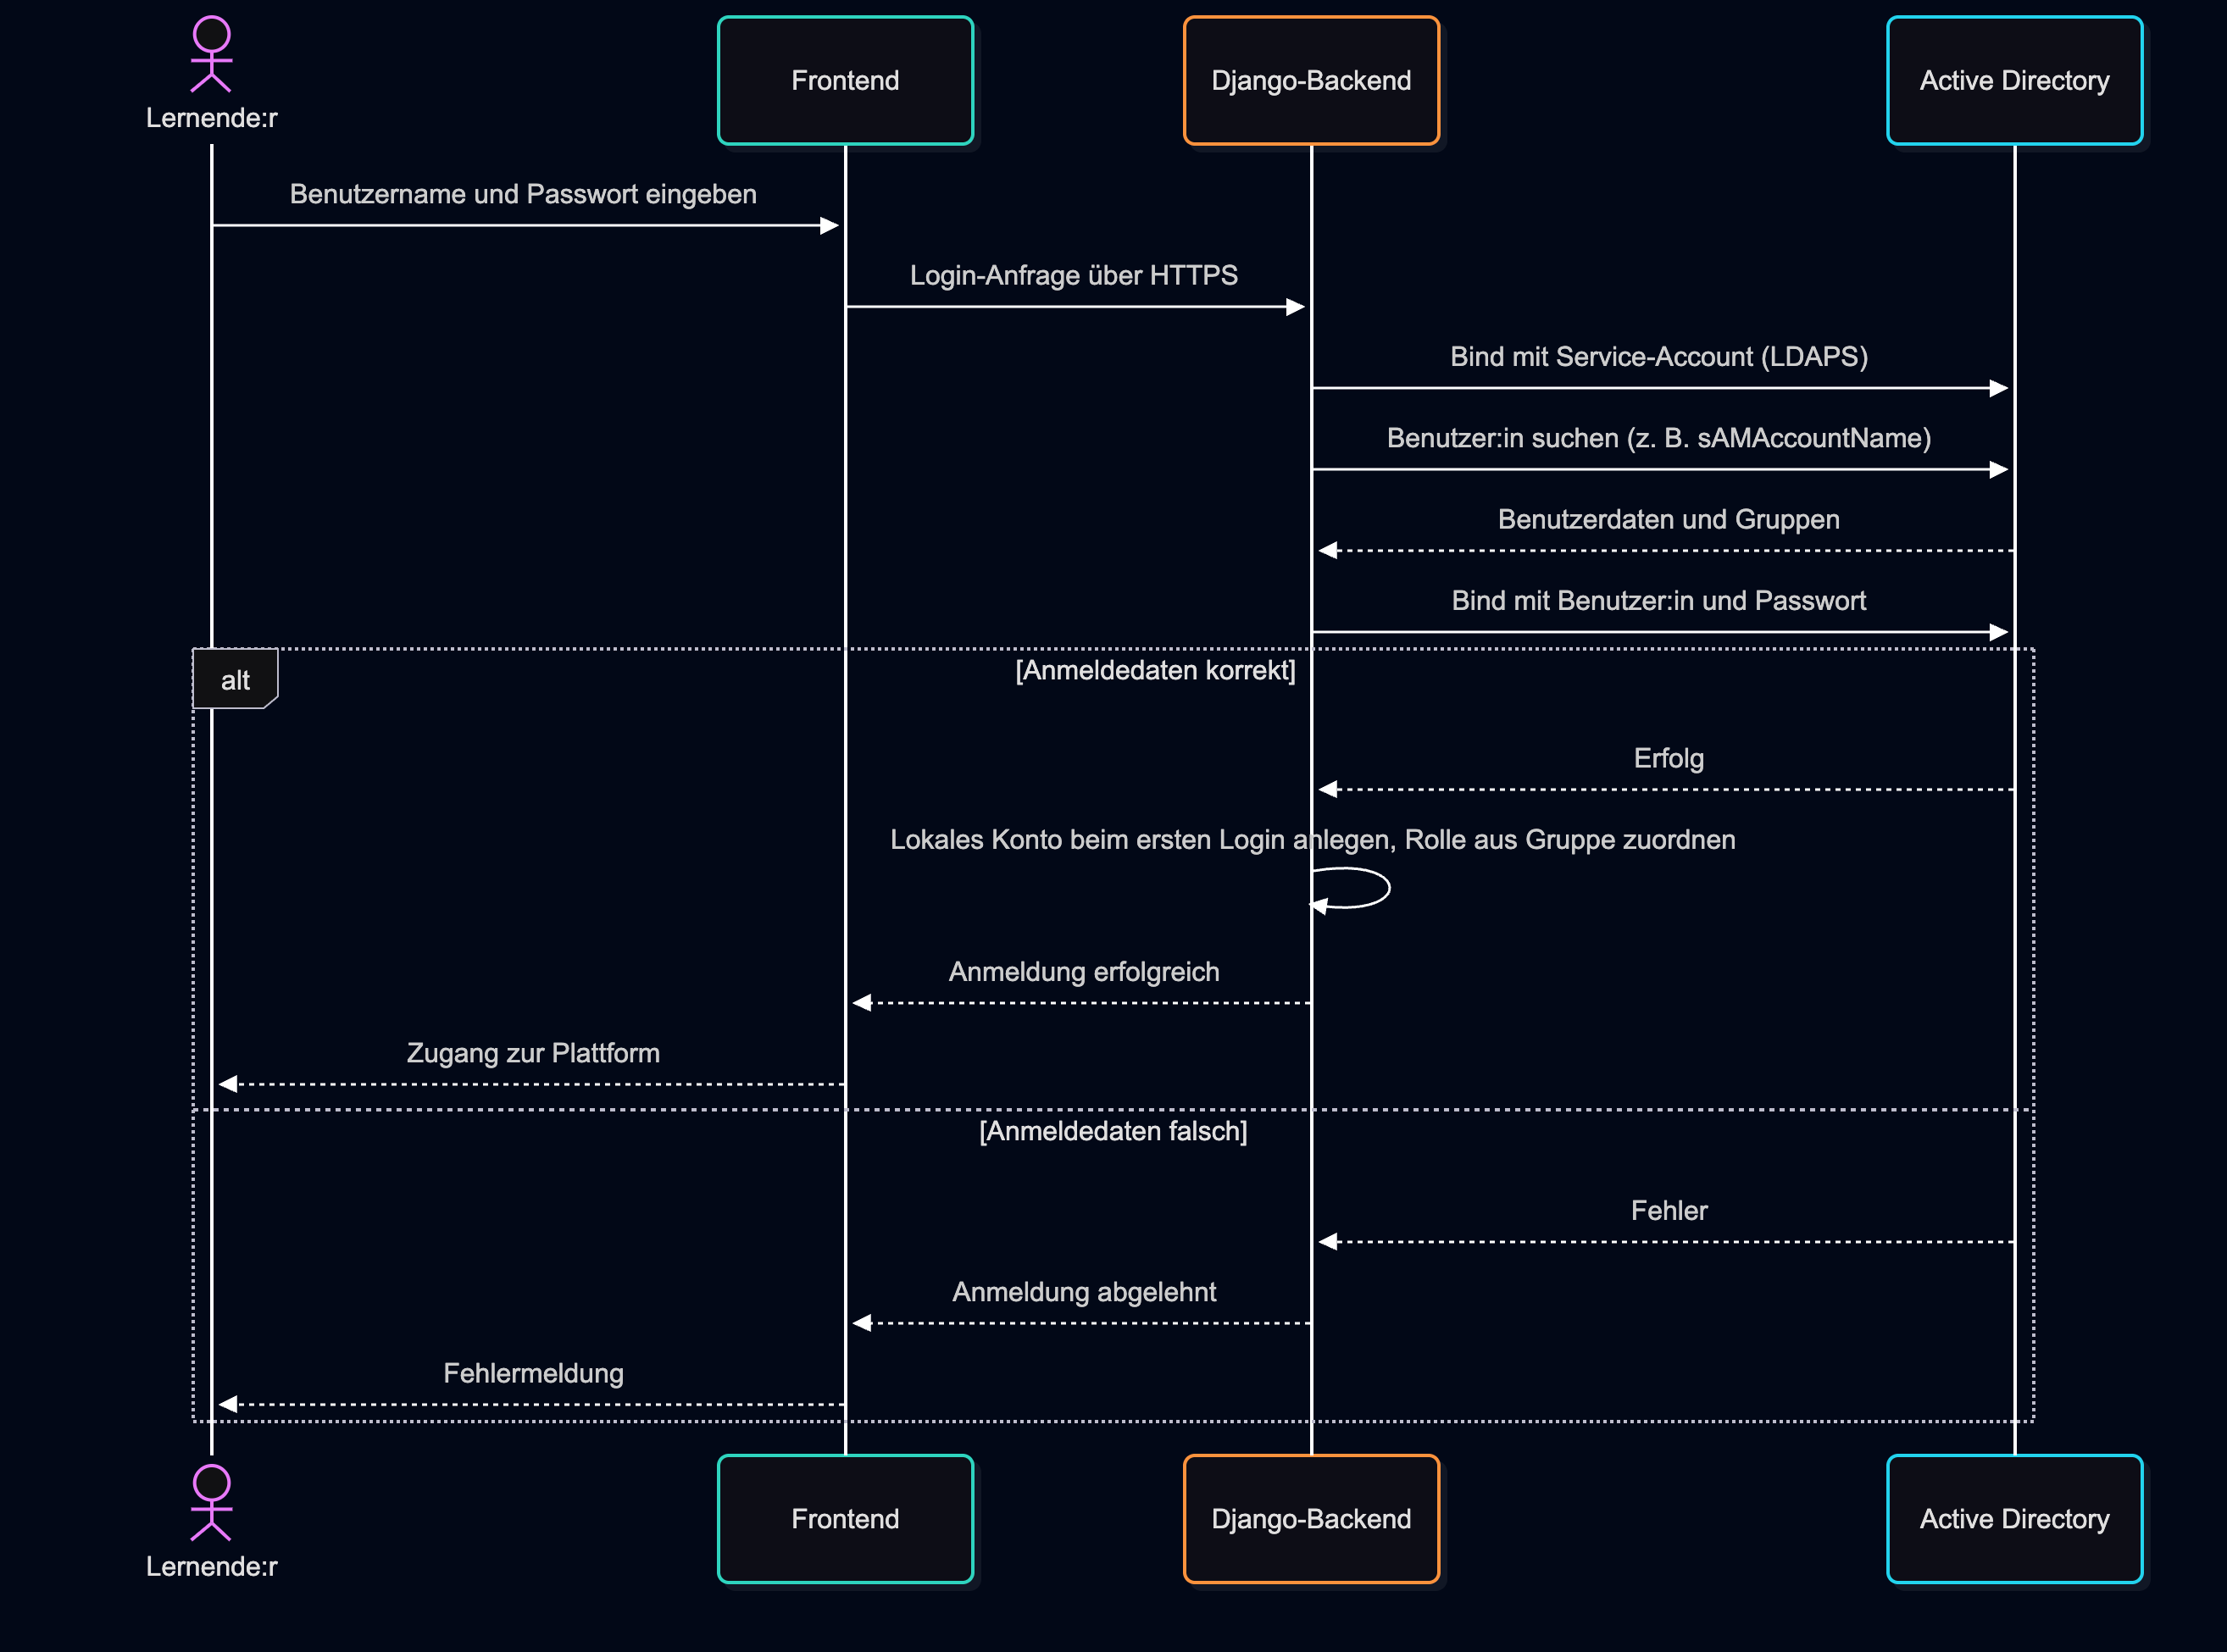
\includegraphics[width=\textwidth,height=0.45\textheight,keepaspectratio]{Bilder/Kumar/Ablauf_der_Authentifizierung_gegen_das_Active_Directory.png}
  \caption{Ablauf der Authentifizierung gegen das Active Directory (eigene Darstellung)}
  \label{fig:ad}
\end{figure}
 
\section{Import und Export von Lerninhalten}
 
Eine Lernplattform braucht Inhalte. Wenn Lehrkräfte jede Lernkarte einzeln eingeben müssen, dauert das zu lang. Mit einem Import und Export können Inhalte in großen Mengen geladen und zwischen Systemen ausgetauscht werden (siehe Abbildung~\ref{fig:importexport}). Dabei sind diese Fragen zu klären:
 
\begin{itemize}
  \item \textbf{Format:} CSV ist einfach, kann aber verschachtelte Inhalte wie Themen, Lernkarten, Antworten und Medien schlecht darstellen. JSON oder ein Paket aus JSON und Mediendateien eignet sich besser.
  \item \textbf{Version:} Eine Versionsnummer im Format verhindert, dass Importe nach Änderungen am Datenmodell unbemerkt falsch laufen.
  \item \textbf{Prüfung:} Importierte Dateien sind nicht vertrauenswürdig. Sie werden auf Aufbau, Größe und Dateitypen geprüft.
  \item \textbf{Keine Duplikate:} Wird dieselbe Datei zweimal importiert, sollen keine doppelten Inhalte entstehen.
  \item \textbf{Fehler:} Ein Import soll ganz oder gar nicht durchgehen (Transaktion). Bei einem Fehler gibt es eine verständliche Liste.
  \item \textbf{Umfang des Exports:} Inhalte und Lernstände werden getrennt betrachtet, weil Lernstände persönliche Daten sind.
\end{itemize}
 
 
\begin{figure}[htbp]
  \centering
  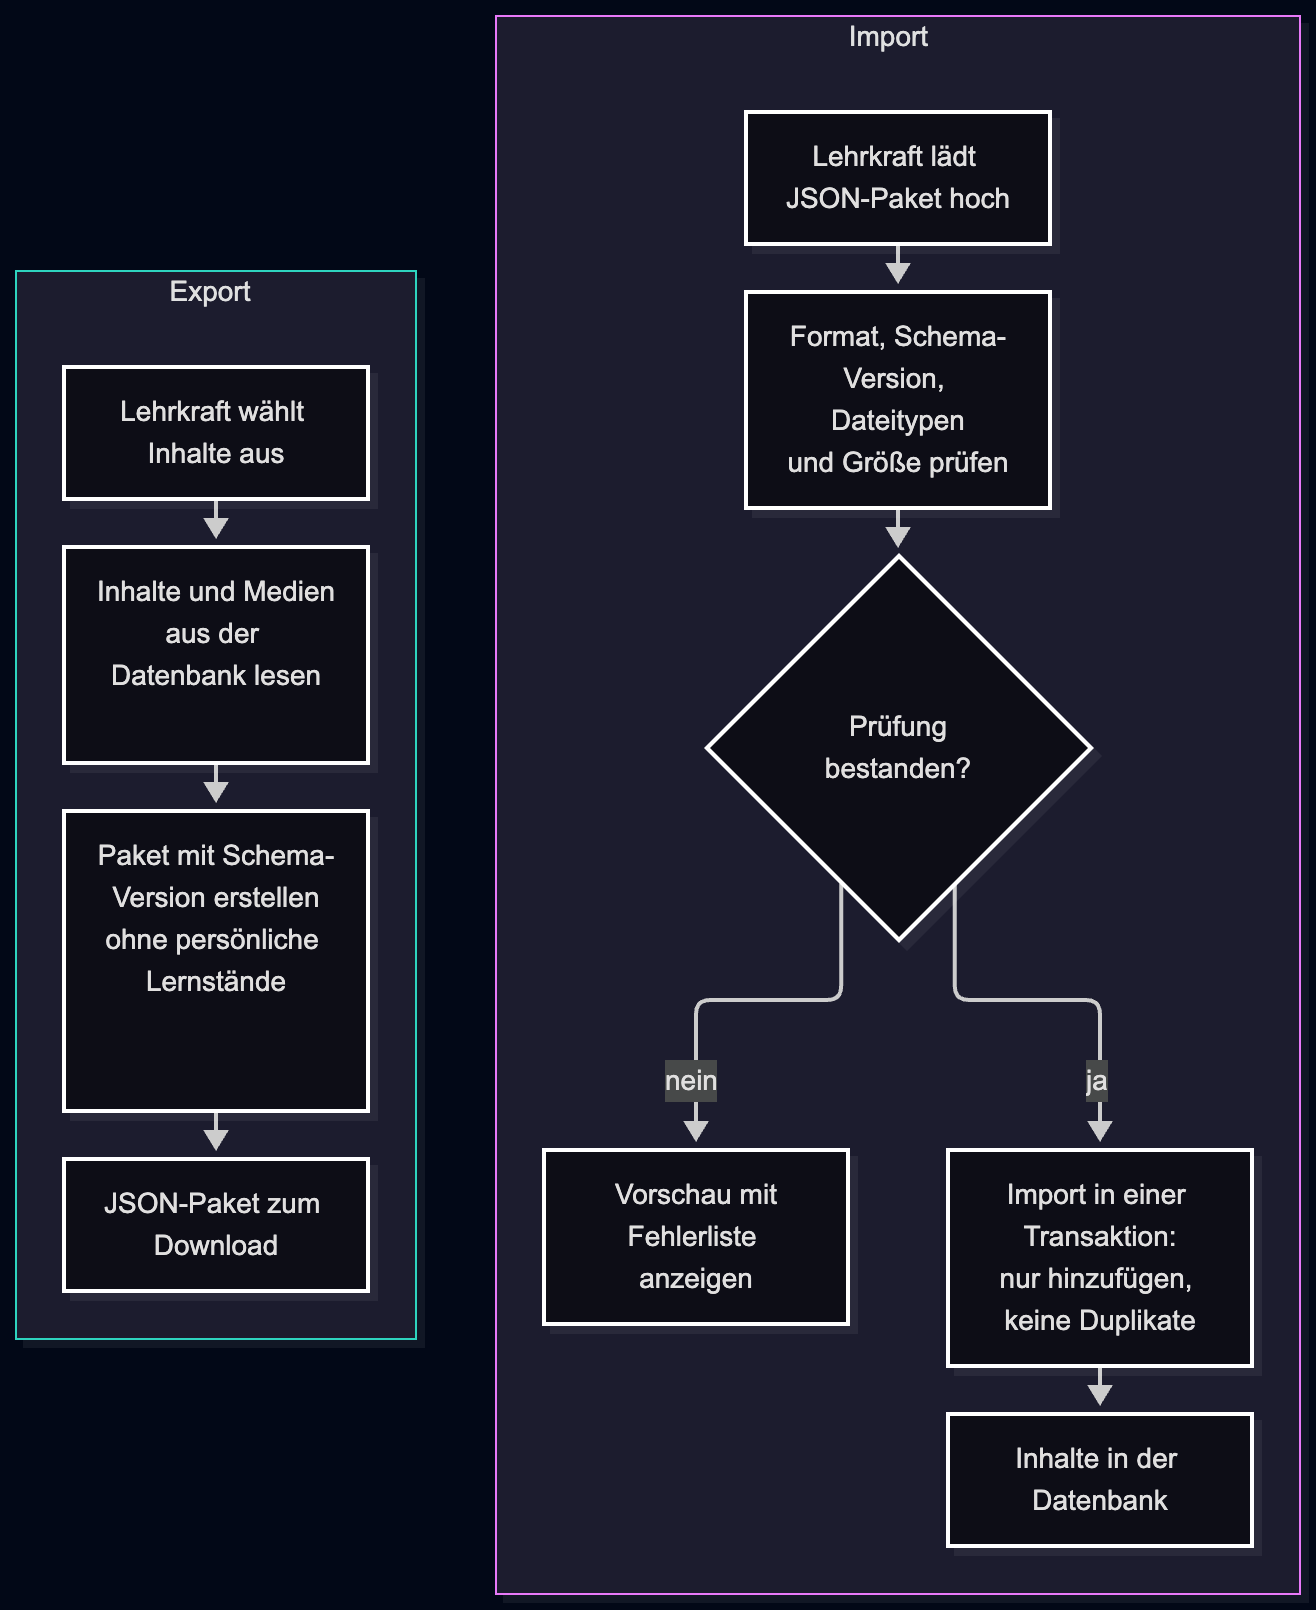
\includegraphics[width=\textwidth,height=0.45\textheight,keepaspectratio]{Bilder/Kumar/Ablauf_von_Import_und_Export.png}
  \caption{Ablauf von Import und Export (eigene Darstellung)}
  \label{fig:importexport}
\end{figure}
 
\section{Sicherheit, Datensicherung und Ausfallsicherheit}
 
\subsection{Sicherheit und Datenschutz}
 
Die Plattform speichert persönliche Daten von Lernenden, zum Beispiel Lernergebnisse. Deshalb gilt die Datenschutz-Grundverordnung (DSGVO). Für die technische Absicherung werden die OWASP Top 10 verwendet. Das ist eine Liste der häufigsten Risiken bei Webanwendungen, zum Beispiel falsche Zugriffsrechte oder Fehler in der Konfiguration \parencite{owasp-top-ten}. Auf der Ebene der Infrastruktur gehören dazu: Die Datenbank ist nur für die Anwendung erreichbar, alle Verbindungen sind mit TLS verschlüsselt, Updates werden regelmäßig eingespielt, Passwörter liegen nicht im Code, und wichtige Ereignisse werden protokolliert. Da das Active Directory auf demselben Server läuft wie die Anwendung, muss der Server besonders gut abgesichert sein.
 
\subsection{Datensicherung und Wiederherstellung}
 
Laut der PostgreSQL-Dokumentation gibt es drei verschiedene Arten, die Datenbank zu sichern: einen SQL-Dump, ein Backup auf Dateisystemebene und die kontinuierliche Archivierung \parencite{postgres-backup-restore}. Die kontinuierliche Archivierung ermöglicht es, die Datenbank auf einen beliebigen früheren Zeitpunkt zurückzusetzen \parencite{postgres-pitr}. Die Sicherungen laufen automatisch und regelmäßig. Zusätzlich gilt die 3-2-1-Regel: drei Kopien auf zwei verschiedenen Speichermedien, eine davon an einem anderen Ort. Auch das Active Directory wird gesichert, damit die Konten bei einem Serverausfall wiederhergestellt werden können. Backups müssen außerdem regelmäßig durch eine Wiederherstellung getestet werden. Ein Backup, das nie getestet wurde, ist keine sichere Absicherung \parencite[Kap.~26]{beyer2016sre}.
 
\subsection{Ausfallsicherheit}
 
Ausfallsicherheit entsteht, wenn wichtige Teile doppelt vorhanden sind und Fehler automatisch erkannt werden. Mit Docker können Container bei einem Fehler automatisch neu gestartet werden. Mehrere Anwendungsinstanzen hinter einem Reverse Proxy wären eine Erweiterung. Jede zusätzliche Absicherung macht das System aber komplizierter und aufwendiger. Deshalb muss sie zum tatsächlichen Bedarf einer Schulplattform passen (Eig.). Auf einem einzelnen Server ist der Server selbst die größte Schwachstelle. Backups und eine dokumentierte Wiederherstellung sind deshalb besonders wichtig.
 
\section{Teststrategie}
 
\subsection{Testarten und Werkzeuge}
 
Die Tests zeigen, ob die Infrastruktur die Anforderungen erfüllt. Es gibt mehrere Arten: \\
Performancetests messen Antwortzeit und Durchsatz bei normaler Last. Lasttests simulieren viele gleichzeitige Benutzer:innen, zum Beispiel eine ganze Klasse, die gleichzeitig einen Test startet. Stresstests erhöhen die Last über das erwartete Maß, um zu sehen, wo das System an seine Grenzen kommt. Stabilitätstests laufen mehrere Stunden und zeigen, ob zum Beispiel der Speicher langsam volläuft. Sicherheitstests suchen nach Schwachstellen und Konfigurationsfehlern und prüfen die Anmeldung \parencite[Kap.~17]{beyer2016sre}. Für Lasttests eignet sich Locust. Dort wird das Verhalten der Benutzer:innen in Python beschrieben \parencite{locust-docs}. Zusätzlich wird getestet, ob sich das System anhand des Repositorys auf einem frischen Server neu aufbauen lässt.
 
\subsection{Messgrößen}
 
Tests sind nur aussagekräftig, wenn vorher festgelegt wird, was gemessen wird. Dafür sind geplant: die Antwortzeit, die Fehlerrate, die Anfragen pro Sekunde und die Auslastung von CPU, Speicher und Datenbank. Die Ergebnisse werden dokumentiert und ausgewertet.
 
\section{Konkurrenzanalyse}
 
\subsection{Positionierung, Ziele und Kriterien}
 
Die Arbeit liegt im Bereich selbst betriebener Lernplattformen für den Schulunterricht, bei denen die Anmeldung zentral läuft. Ziel ist eine Infrastruktur, die sich jederzeit neu aufbauen lässt, mitwächst, die Anmeldung über ein Active Directory erlaubt und Lerninhalte offen austauschbar macht. Daraus ergeben sich vier Kriterien: Skalierbarkeit und Betrieb, Anbindung an Verzeichnisdienste, Qualität und Offenheit von Import und Export und Kontrolle über die eigenen Daten.
 
\subsection{Auswahl der Konkurrenz}
 
Auf der ersten Ebene, also mit ähnlichem Zweck und Einsatz, wurde Moodle gewählt. Moodle ist eine Lernplattform, die Schulen und Hochschulen selbst betreiben. Auf der zweiten Ebene wurden die Lernkarten-Programme Anki und Quizlet untersucht. Sie erfüllen dieselbe Aufgabe, nämlich Lernen mit Karten, aber auf andere Weise: Anki läuft lokal, Quizlet als Cloud-Dienst. Als Beispiel für eine Django-Anwendung mit AD-Anbindung dient zusätzlich Review Board. Die Analyse stützt sich auf die öffentliche Dokumentation der Hersteller und nicht auf eigene Langzeittests. Screenshots der untersuchten Funktionen kommen zur besseren Nachvollziehbarkeit in den Anhang.
 
\subsection{Moodle}
 
\textbf{Stärken.}
\begin{enumerate}
  \item Skalierbarkeit: Die Schichten der Anwendung sind klar getrennt. Dadurch kann Moodle auf mehrere Webserver verteilt werden, die dieselbe Datenbank und denselben Dateibereich benutzen \parencite{moodle-performance}.
  \item Verzeichnisanbindung: Moodle kann Anmeldungen über LDAP prüfen, ausdrücklich auch mit Microsoft Active Directory \parencite{moodle-ldap}.
  \item Passwörter: Die Passwörter der LDAP-Benutzer:innen müssen nicht in Moodle gespeichert werden \parencite{moodle-ldap}.
\end{enumerate}
 
\textbf{Schwächen.}
\begin{enumerate}
  \item Viel Einrichtungsaufwand: Auch bei gleichem Servertyp wie AD kann jede Installation eine ganz andere Verzeichnisstruktur haben. Die Einstellungen müssen deshalb jedes Mal angepasst werden \parencite{moodle-ldap}.
  \item Einschränkungen: Laut Dokumentation funktionieren bei Active Directory manche Vorgänge nicht, zum Beispiel das Aktualisieren von Daten im Verzeichnis. Die Anmeldung selbst ist davon nicht betroffen \parencite{moodle-ldap}.
  \item Viel Feintuning: Im Betrieb sind manuelle Anpassungen nötig, zum Beispiel bei den Apache-Einstellungen. Bei sehr großen Systemen mit Lastverteilung wird die Leistung von Dateispeicher und Cache wichtig \parencite{moodle-performance}.
\end{enumerate}
 
\textbf{Chancen.} Eine schlankere Plattform kann den Betrieb einfacher machen, indem die AD-Einstellungen fertig dokumentiert sind und alles als Container versioniert im Repository bereitgestellt wird.
 
\subsection{Anki}
 
\textbf{Stärken.}
\begin{enumerate}
  \item Austauschformat: Ein Deckpaket (.apkg) enthält Karten, Notizen, Notiztypen sowie Ton- und Bilddateien in einer einzigen Datei \parencite{anki-exporting}.
  \item Import fügt nur hinzu: Beim Import eines Deckpakets werden die Inhalte der Sammlung hinzugefügt und nichts überschrieben \parencite{anki-exporting}.
  \item Inhalt und Lernstand getrennt: Beim Export kann man die Lerninformationen weglassen, damit ein Deck sauber weitergegeben werden kann \parencite{anki-exporting}.
\end{enumerate}
 
\textbf{Schwächen.}
\begin{enumerate}
  \item Gefährlicher Vollimport: Wird eine Collection-Datei (.colpkg) importiert, werden alle aktuellen Karten gelöscht und durch den Inhalt der Datei ersetzt \parencite{anki-exporting}.
  \item Eingeschränkter Rückimport: Ein Textexport kann nur dann zuverlässig wieder importiert werden, wenn das erste Feld nicht verändert wird \parencite{anki-exporting}.
  \item Austausch per Datei: Inhalte werden von Hand als Dateien weitergegeben. Eine zentrale Benutzer- und Rechteverwaltung für den Schulbetrieb kommt in den untersuchten Teilen der Dokumentation nicht vor.
\end{enumerate}
 
\textbf{Chancen.} Die Ideen vom Import, der nur hinzufügt, und vom getrennten Export von Inhalt und Lernstand lassen sich in einem zentralen System mit Rechteverwaltung und einer Vorschau vor dem Import besser umsetzen.
 
\subsection{Quizlet}
 
\textbf{Stärken.}
\begin{enumerate}
  \item Export eigener Sets: Begriffe und Definitionen von eigenen Sets können exportiert werden \parencite{quizlet-exporting}.
  \item Freigabe: Das Hilfecenter beschreibt Einstellungen für die Sichtbarkeit von Sets, für Bearbeitungsrechte und für Passwortschutz \parencite{quizlet-sharing}.
  \item Komfort: Sets können gedruckt, eingebettet und in den mobilen Apps offline gelernt werden \parencite{quizlet-sharing}.
\end{enumerate}
 
\textbf{Schwächen.}
\begin{enumerate}
  \item Eingeschränkter Export: Bilder können aus Urheberrechtsgründen nicht exportiert werden, und kopierte Sets lassen sich gar nicht exportieren \parencite{quizlet-exporting}.
  \item Premium-Beschränkungen: In der kostenlosen Version können Sets, die mit Premium-Funktionen erstellt wurden, nicht kopiert und gespeichert werden \parencite{quizlet-copying}.
  \item Abhängigkeit vom Anbieter: Die Inhalte liegen auf der Plattform des Anbieters. Die Schule hat keinen Einfluss auf Betrieb und Datenspeicherung.
\end{enumerate}
 
\textbf{Chancen.} Eine selbst betriebene Plattform kann Inhalte vollständig mit Medien exportierbar halten, und die Daten bleiben bei der Schule.
 
\subsection{Gesamtvergleich}
 
\begin{center}
\small
\begin{tabular}{|p{2.0cm}|p{3.4cm}|p{3.6cm}|p{4.0cm}|}
\hline
\textbf{Konkurrenz} & \textbf{Wichtigste Stärke} & \textbf{Wichtigste Schwäche} & \textbf{Folge für die Arbeit} \\ \hline
Moodle & Lastverteilung, LDAP/AD & Viel Einrichtung und Feintuning & Zustandslose Anwendung, aber einfache, dokumentierte Konfiguration \\ \hline
Anki & Austauschpaket, Import fügt nur hinzu & Vollimport löscht Karten, Austausch von Hand & Austauschformat mit Medien, nur hinzufügender Import \\ \hline
Quizlet & Einfacher Export eigener Sets & Kein Export von Bildern, abhängig vom Anbieter & Offenes, vollständiges Exportformat, eigene Datenhaltung \\ \hline
\end{tabular}
\end{center}
Als Vorbild für die AD-Anbindung in einer Django-Anwendung dient Review Board. Laut Dokumentation wird das AD-Backend über Domänenname, Suchbasis und TLS eingestellt. Es findet Domänencontroller über DNS und legt Benutzer:innen, die nur im AD vorhanden sind, beim ersten Login in der lokalen Datenbank an \parencite{reviewboard-ad}.
 
\section{Fazit der Vorfeldanalyse}
 
\subsection{Getroffene Entscheidungen}
 
Aus der Vorfeldanalyse, der Aufgabenstellung und der Konkurrenzanalyse ergeben sich diese Entscheidungen:
 
\begin{description}
  \item[DE-1 Docker Compose.] Die Plattform läuft in Containern, die mit Docker Compose gemeinsam beschrieben und gestartet werden (Reverse Proxy, Django mit Gunicorn, Datenbank). Die Beschreibung liegt zusammen mit dem Code in einem GitHub-Repository, die Zugangsdaten in Umgebungsvariablen. Die Entscheidung fiel auf Docker, weil sich die Umgebung damit jederzeit auf einem neuen Server aufbauen lässt und der Einrichtungsaufwand kleiner wird, der bei Moodle auffällt. Auf Kubernetes wird verzichtet, weil der Aufwand für dieses Projekt zu groß wäre.
  \item[DE-2 Zustandslose Anwendung.] Die Anwendung ist so gebaut, dass bei Bedarf weitere Instanzen laufen können, ohne Sitzungen oder Dateien bei sich zu speichern. Für den Anfang läuft eine Instanz. Das ist dem Skalierungsmodell von Moodle nachempfunden.
  \item[DE-3 PostgreSQL.] Die Datenbank läuft in einem eigenen Container, speichert ihre Daten außerhalb des Containers und ist nur für die Anwendung erreichbar. Ausschlaggebend waren die sichere Verarbeitung von Transaktionen, die Unterstützung durch Django und die guten Backup-Möglichkeiten.
  \item[DE-4 Datenbankstruktur.] \Jai definiert die Struktur der Datenbank als ER-Diagramm mit Tabellenbeschreibung, ausgehend vom Entwurf von \Luca. Der Lernfortschritt wird berechnet und nicht gespeichert. Die Datenbank sichert Eindeutigkeit und Beziehungen über Schlüssel ab, zusammengehörige Änderungen laufen in einer Transaktion, und für die häufigste Abfrage (fällige Lernkarten) ist bei Bedarf ein Index vorgesehen. Änderungen laufen über Migrationen im Repository. Die Umsetzung im Backend bleibt bei \Luca.
  \item[DE-5 Eigenes Active Directory mit LDAPS.] Weil die Schule keinen Zugriff auf ihr Active Directory gibt, wird ein eigenes AD eingerichtet, voraussichtlich auf demselben Server wie die Anwendung. Die Anmeldung läuft verschlüsselt gegen dieses AD, mit einem Service-Account mit möglichst wenigen Rechten. AD-Gruppen werden Rollen zugeordnet, und Benutzer:innen werden beim ersten Login lokal angelegt, nach dem Vorbild von Review Board. Ein lokaler Administrationszugang bleibt als Notfallweg. Das eigene AD enthält Testkonten und dient gleichzeitig als Test-Verzeichnis für Entwicklung und Tests.
  \item[DE-6 Offenes Austauschformat.] Lerninhalte werden als JSON-Paket mit Versionsnummer und Medienordner ausgetauscht. Der Import fügt nur hinzu, erzeugt keine Duplikate, läuft als Transaktion und prüft die Dateien. Exportiert werden standardmäßig nur Inhalte und keine persönlichen Lernstände. Die Entscheidung stützt sich auf die Stärken von Anki und die Schwächen von Quizlet.
  \item[DE-7 Backup-Konzept.] Geplant sind regelmäßige automatische Sicherungen der Datenbank und des Active Directory, die Aufbewahrung nach der 3-2-1-Regel und regelmäßige, protokollierte Wiederherstellungstests.
  \item[DE-8 Gestaffelte Tests.] Lasttests mit Locust mit realistischen Szenarien, festgelegte Messgrößen, ein Stabilitätstest über mehrere Stunden und eine Sicherheitsprüfung nach den OWASP Top 10. Zusätzlich wird der Neuaufbau aus dem Repository getestet. Die Ergebnisse werden dokumentiert und fließen in Verbesserungen ein.
\end{description}
 
\subsection{Risiken und offene Fragen}
 
\begin{itemize}
  \item \textbf{Schulserver:} Es ist noch offen, ob die Schule einen Server bereitstellt. Wenn nicht, läuft die Plattform lokal.
  \item \textbf{Alles auf einem Server:} Anwendung, Datenbank und Active Directory auf demselben Server sind einfacher einzurichten, aber nicht die empfohlene Praxis. Ein Ausfall oder ein Angriff betrifft alles zugleich.
  \item \textbf{Eigenes statt Schul-AD:} Das Projektziel einer zentralen Anmeldung über das Schulnetzwerk wird durch ein eigenes AD ersetzt. Dieses enthält nur Testkonten und ist nicht mit den echten Schulkonten verbunden.
  \item \textbf{Einarbeitung in Docker:} Docker und Docker Compose müssen im Team erst eingerichtet und verstanden werden. Dafür muss Zeit eingeplant werden.
  \item \textbf{Offene Punkte der Datenbankstruktur:} Offen ist, ob auch Testaufgaben einen Wiederholungsstatus bekommen, wie das Lernergebnis umgesetzt wird (ein Modell oder zwei) und ob Daten der Gamification-Elemente gespeichert werden. Ebenso offen ist das Löschverhalten bei Benutzer:innen. Das wird mit \Luca und \Jakob geklärt.
  \item \textbf{Änderungen an der Struktur:} Backend und Frontend hängen von der Datenbankstruktur ab. Änderungen müssen deshalb früh im Team abgestimmt werden.
  \item \textbf{Anzahl der Benutzer:innen:} Wie viele Personen gleichzeitig online sein werden, ist nicht bekannt und muss für die Lasttests angenommen werden.
  \item \textbf{Abstimmung im Team:} Die Aufteilung beim Backend (LDAP-Einstellungen, Umsetzung der Datenbankstruktur, Import- und Export-Logik) und beim Frontend (Oberfläche für Import und Export) wird mit \Luca und \Jakob genauer geklärt.
\end{itemize}
 
\section*{Abbildungsverzeichnis (\Jai)}
 
\begin{itemize}
  \item Abb.~\ref{fig:architektur}: Architekturübersicht der Infrastruktur (eigene Darstellung)
  \item Abb.~\ref{fig:er}: Entwurf der Datenbankstruktur als ER-Diagramm (eigene Darstellung)
  \item Abb.~\ref{fig:ad}: Ablauf der Authentifizierung gegen das Active Directory (eigene Darstellung)
  \item Abb.~\ref{fig:importexport}: Ablauf von Import und Export (eigene Darstellung)
\end{itemize}